\documentclass[12pt, letterpaper]{report}
\usepackage[utf8]{inputenc}
\usepackage[T1]{fontenc} 
\usepackage[spanish]{babel}
\usepackage{color}
\usepackage{verbatim} 
\usepackage{longtable} 
\usepackage{graphicx}
\usepackage{listings} % insertar código
\usepackage{url} % hyperlinks
\usepackage{hyperref} % navegación en PDF

%-------------------------------
% Path de imagenes
%-------------------------------

\graphicspath{ {imgs/} }

%-------------------------------
% Formato para código
%-------------------------------

\definecolor{codegreen}{rgb}{0,0.6,0}
\definecolor{codesoftgreen}{rgb}{0,0.5,0}
\definecolor{codeblue}{rgb}{0.,0.,0.6}
\definecolor{codered}{rgb}{0.9,0,0.2}
\definecolor{backcolour}{rgb}{0.95,0.95,0.92}

\lstset{language=c}
\lstset{ %
  basicstyle=\footnotesize,        % tamaño de fuente
  breakatwhitespace=false,         
  breaklines=true,                 
  captionpos=b,                    
  keywordstyle=\color{codeblue},
  stringstyle=\color{codesoftgreen},
  commentstyle=\color{codegreen},
  numberstyle=\color{codered},
  morecomment=[l][\color{magenta}]{\#},
  frame=single,                    % borde
  keepspaces=true,                 
  language=c,                 % lenguaje
}

%-------------------------------
% Documento
%-------------------------------

\title{Información preliminar a \\ SuperCollider: curso introductorio}
\author{Darien Brito}

\begin{document}

\begin{titlepage}
\maketitle
\end{titlepage}

\begin{abstract}
Este artículo sirve de preámbulo a conceptos claves para entender con facilidad los vídeos del curso. Si no tienes ninguna experiencia previa con programación, asegúrate de leer la información en este documento antes de empezar el tutorial.
\end{abstract}

\tableofcontents{}
\listoffigures
\pagestyle{plain}

\chapter{Coding}

\section{¿Qué es coding?}

Este tutorial trata sobre el lenguaje de programación SuperCollider y sus capacidades para crear sonidos y música. Estarás por tanto lidiando con código como método creativo. La práctica de escribir código es denominada ``coding''. Ten en claro por tanto que todo lo que creas está basado en texto. Mientras más rápido escribas y entiendas las palabras necesarias para ejecutar instrucciones con este texto, mejor. Por esta razón, el curso es un tanto agresivo, conciso y rápido, a fin de forzarte a escribir inmediatamente pequeños programas, incluso si no los entiendes del todo. 

El código de computadoras es intimidante al principio y puede ser frustrante no poder entender inmediatamente su modo de operación, dado que es un lenguaje un tanto antinatural para la mayoría de las personas. Piensa sin embargo que es un lenguaje creado por seres humanos para seres humanos, \textit{ergo} cualquier persona es capaz de aprenderlo con el entrenamiento adecuado. La mejor forma de hacerlo es copiando, cambiando parámetros, cometiendo errores y construyendo tus propias instrucciones en base a lo que vas aprendiendo. 

La razón por la que es interesante aprender a programar es que nos da una capacidad creativa enorme y un poder expresivo gigantesco. En la actualidad, el código ha pasado a ser una herramienta muy cercana a la práctica artística y hay toda una nueva corriente de arte creada con medios digitales expresados con código. En audio, en concreto, entender los principios de síntesis a nivel de programación te permitirán dominar técnicas en cualquier otra plataforma y a generar cientos de sonidos con pequeños cambios de parámetros en lugar de usar incontables horas moviendo diales y haciendo click en botones.

Para toda tarea necesitamos tener un conocimiento básico de ciertas nociones antes de comenzar a realizar la tarea en sí. Imagina que estás por ejemplo cocinando algo tan simple como un plato de spagetti. El mínimo conocimiento previo que necesitas para hacer este plato es saber hervir el agua, debes tener los productos adecuados, como la pasta, cebollas, ajo y además tener las herramientas adecuadas, como una olla, una sartén, un escurridor, un plato y utensillos. Con SuperCollider, es exactamente lo mismo. \underline{Antes de hacer sonidos}, necesitamos primero saber qué productos tenemos disponibles y que herramientas son las adecuadas para cada tarea. Por esto, sé paciente y trata de entender los bloques básicos de programación que se presentan en el curso antes de generar nuestro primer sonido. 

\section{¿Cómo aprender?}

Como he sugerido ya, la mejor forma de aprender a programar es copiando\footnote{Asegúrate de escribir lo que copias y no hacer ``copy-paste''} y haciendo pequeños cambios en el código. Por ejemplo, en el primer capítulo de este tutorial verás el programa ``¡Hola Mundo!''. El código para este programa se ve así:

\begin{lstlisting}
``Hola mundo!''.postln;
\end{lstlisting}

Inmediatamente puedes probar cambiando algo en este código:

\begin{lstlisting}
``Chao mundo!''.postln;
\end{lstlisting}

Esta pequeña alteración, si ejecutada, te permite concluir que lo que va entre comillas es el texto a ser impreso y que probablemente no importa realmente lo que vaya escrito dentro:

\begin{lstlisting}
``Esto puede ser cualquier cosa''.postln;
\end{lstlisting}

Puedes continuar viendo más elementos en esta pequeña línea. ¿Qué pasa si alteras el punto por una coma?

\begin{lstlisting}
``Esto puede ser cualquier cosa'',postln; 
\end{lstlisting}

¡Error! ¿Y si alteramos postln?

\begin{lstlisting}
``Esto puede ser cualquier cosa''.imprimir; 
\end{lstlisting}

¡Otro error¡ Mmm... 

Este ejercicio tan simple ha sido capaz de enseñarnos ya varias cosas muy útiles. Podemos deducir por ejemplo que el punto en la instrucción es necesario y que no puede ser por ejemplo una coma, y que ``postln'' es una palabra especial para imprimir en la consola y por tanto deben existir otras palabras especiales para realizar acciones diferentes. 

Pese a que puedes pensar que esto no tiene nada que ver con hacer sonidos o música, resulta que nos ayuda a comprender cómo funciona una computadora ¡Verás que cuando escribas código para generar audio saber lo que este pequeño programa hace y por qué funciona es muy útil!

\section{¿Qué es un repositorio?}

Todo el código de soporte para este curso está disponible en un repositorio online alojado en el sitio Github. Ok, ¿pero qué es un repositorio?

Un repositorio es un archivo en donde se almacena información digital. En nuestro caso, es el lugar en donde todo el material de soporte para el curso se aloja. Este material contiene:

\begin{itemize}
\item El código de cada capítulo
\item Transcripciones de los vídeos 
\item El código LaTeX para generar este documento
\item Este PDF
\item El código para generar los sonidos de introducción de cada vídeo
\end{itemize}

Para acceder al repositorio puedes hacer click en este \href{https://github.com/DarienBrito/Quadro_SCIntro} {\textbf{link}} o puedes ir a la siguiente dirección:

\small{
\begin{verbatim}
https://github.com/DarienBrito/Quadro_SCIntro
\end{verbatim}
}

\section{¿Qué es Open Source?}

\textit{Open Source} es la denominación en inglés para referirse a software cuyo código fuente es libre, es decir, que puede ser visto y modificado por cualquier usuario. 

A diferencia de los programas comunes, que funcionan como una caja negra que podemos usar pero a cuyo código fuente no podemos acceder, proyectos de código libre hacen todo disponible sin ninguna restricción. SuperCollider es un proyecto \textit{open source}, así como el repositorio para este curso.

\section{¿Qué es GitHub?}

De acuerdo a la explicacion en la página oficial de Git:

\begin{quote}
GitHub es una plataforma de desarrollo colaborativo de software para alojar proyectos utilizando el sistema de control de versiones Git.
\end{quote}

Una gran cantidad de proyectos \textit{open source} se alojan en GitHub porque es una herramienta muy útil para compartir y modificar código y documentos online. Si quieres aprender más al respecto, puedes leer la documentación en este \href{http://conociendogithub.readthedocs.io/en/latest/data/introduccion/} {\textbf{link}} o yendo a la siguiente dirección:

\begin{verbatim}
http://conociendogithub.readthedocs.io/en/latest/data/introduccion/
\end{verbatim} 



\chapter{Música con programación}

\section{Máquinas para música}

Podrías preguntarte: ¿por qué usar un lenguaje de programación para hacer música? e inmediatamente responderte con otra pregunta: ¿por qué no?

Antes de que fuera práctico hacer música electrónica con computadoras, los medios para generar y medir sonidos consistían en circuitos analógicos conectados con cables y controlados con niveles de voltaje. Los primeros usuarios de dichas máquinas no fueron músicos o compositores, sino científicos para quienes eran necesarios ciertos medios a fin de realizar experimentos. 

El uso de máquinas electrónicas para hacer música fue impulsado gracias a los esfuerzos de compositores como \href{https://es.wikipedia.org/wiki/Pierre_Schaeffer} {\textbf{Pierre Schaeffer}} o \href{https://es.wikipedia.org/wiki/Karlheinz_Stockhausen}{\textbf{Karlheinz Stockhausen}}, que dedicaron gran parte de su práctica artística a expandir posibilidades sonoras y a desarrollar junto con ingenieros nuevos instrumentos electrónicos.   

Posteriormente, alrededor de los años 60, pioneros como \href{https://es.wikipedia.org/wiki/Robert_Moog}{\textbf{Bob Moog}} y \href{https://es.wikipedia.org/wiki/Don_Buchla}{\textbf{Don Buchla}} produjeron máquinas analógicas específicamente para propósitos musicales y popularizaron su uso en todo tipo de géneros. 

Lógicamente, una vez el poder de procesamiento y las interfaces para computadoras evolucionaron lo suficiente, la producción de música electrónica comenzó a trasladarse a medios digitales. Pioneros en este campo como \href{https://es.wikipedia.org/wiki/Gottfried_Michael_Koenig} {\textbf{Gottfried Michael Koenig}} y \href{https://es.wikipedia.org/wiki/Iannis_Xenakis} {\textbf{Iannis Xenakis}} realizaron conceptos e ideas radicales que transformaron el modo en el que escuchamos y producimos música.

\section{Medios}

Existen numerosos predecesores de los programas y aplicaciones para audio actuales, entre ellos Kyma\footnote{http://kyma.symbolicsound.com/}, Common Music\footnote{http://commonmusic.sourceforge.net/} y CSound\footnote{http://csound.github.io/}, que fueron creados en los años 80. Estos programas son ambientes de programación y siguen en uso hoy. El paradigma para hacer música en computadoras cambió con la introducción de la línea de tiempo tradicional e interfaces más amigables como en programas como Ableton Live, Logic o Pro Tools.

En esencia, estos programas no son sino código disfrazado con interfaces más accesibles. La desventaja es que, si creamos música exclusivamente con estas herramientas y tenemos una idea que no forma parte del programa, ¡no podemos realizar nuestra idea! Usar un lenguaje de programación para hacer música y sonidos nos da libertad absoluta para implementar ideas que de otra forma no son posibles. 

Programar no es para todo el mundo y eso está bien, porque a veces no necesitamos profundizar tanto en algo para tener resultados. Sin embargo, si sientes que los métodos tradicionales para realizar música no te satisfacen, \href{http://supercollider.github.io/}{\textbf{SuperCollider}} es una herramienta perfecta para experimentar.

\section{Música con computadoras}

Existen obvias y no tan obvias diferencias entre hacer música con medios puramente acústicos, medios electrónicos analógicos y computadoras. ¿Qué es especial acerca de hacer música con computadoras?

\begin{itemize}
\item Velocidad de ejecución
\item Precisión
\item Exploración de ideas formalizadas
\item Experimentación con varios modelos compositivos
\item Experimentación con procesos generativos
\item Creación y re-utilización de instrumentos sonoros
\end{itemize}

En esencia, hacer cosas que sin una computadora son imposibles de realizar. En el proceso, la computadora puede tomar vario roles. Podría ser por ejemplo:

\begin{itemize}
\item Una herramienta para composición
\item Un generador de material sonoro
\item Un asistente para organizar material sonoro
\item Un asistente para transformación de material (efectos)
\item Un performer automático, supervisado o no
\item Un medio para analizar música 
\item Un instrumento musical 
\item Un medio para reproducir música
\end{itemize}

\section{Programación y música}

Cuando comenzamos a trabajar con música generada con computadoras, nuestras percepciones cambian y eventualmente desarrollamos un nuevo oído musical. Sonidos que antes no nos parecían especiales comienzan a interesarnos y nuevas estructuras sonoras se forman en nuestra cabeza. Nuestra sensitividad también muta, poco a poco somos capaces de escuchar más y mejor, pues los detalles que podemos controlar y a los que tenemos que prestar atención al componer música digital son en muchos casos más finos y sutiles que al lidiar con instrumentos convencionales. Nuevas preguntas aparecen y nuestras pre-concepciones sobre lo que es musical se aligeran. 

Por ejemplo podemos empezar a preguntarnos: ¿hay diferencias entre componer música y componer sonidos? Sin notas definidas, ¿tiene sentido concebir música más alla de escalas y ritmos? ¿podemos controlar sonidos en niveles de tiempo menores al de la nota más rápida? Citando al compositor islandés Bjarni Gunnarsson, quien es a propósito un brillante usuario de SuperCollider:

\begin{quote}
Could we think of the sounds a music creates instead of which music sounds create? \footnote{¿Sería posible pensar en los sonidos que una música crea en lugar de qué música los sonidos crean?}
\end{quote}

Generar arte con algoritmos tiene consecuencias en nuestra forma de pensar y nuestra estética, por esto no es soprendente que nuestro trabajo cambie, a veces drásticamente, una vez que dominamos cierta herramienta. En nuestro caso, esta herramienta es SuperCollider.



\chapter{SuperCollider}

\section{¿Qué es SuperCollider?}

SuperCollider es un lenguaje de programación general orientado a objetos. Esto significa que usando texto y expresiones determinadas, podemos realizar cualquier tarea computacional usando un paradigma de jerarquias y herencia de clases. Su objetivo principal es sintetizar audio en tiempo real y componer sonidos y obras musicales mediante algoritmos. 

Dentro del contexto de software para síntesis de audio, es uno de los más versátiles y poderosos ambientes de programación gracias a su sintaxis compacta y a la inmensidad de aplicaciones y extensiones generadas por sus usuarios. SuperCollider es software de código libre y es absolutamente gratuito. Fue originalmente creado por James McCartney y esta constantemente evolucionando gracias a su muy activa comunidad. 

Es difícil explicar lo que SuperCollider es capaz de hacer precisamente por la inmensidad de opciones que ofrece. Algunos ejemplos de aplicaciones comunes:

\begin{itemize}
\item Síntesis de audio
\item Composiciones automáticas
\item Creación de instrumentos digitales
\item Live coding
\item Creación de música generativa
\item Creación de instalaciones sonoras
\item Interacción con interfaces y sensores
\item Desarrollo de software para aplicaciones científicas
\item Musíca en red
\end{itemize}

Sin embargo, podemos realizar proyectos menos comunes y más atrevidos. Por dar un ejemplo bizarro: digamos que queremos sonificar todos los tweets de una cuenta de Twitter en base a ciertas reglas propias y queremos que otras computadoras alrededor del mundo reconozcan mensajes que les digan cuando tocar ciertos sonidos en base a estos tweets. Mientras hacemos esto, queremos enviar datos a diez microcontroladores ubicados alrededor del mundo, que reaccionan de acuerdo al análisis de la señal del mercado de acciones de Google durante los últimos diez años. Cada uno de estos motores toca una campana en diferentes ciudades del mundo, sincronizadas mediante nuestra laptop en casa... ¿cómo haríamos todo esto con software estándar? Pues bien, para esto podemos usar SuperCollider.

Como ves, las aplicaciones son difíciles de definir y engloban una gran cantidad de posibilidades. A modo de ejemplo, puedes ir al link: \href{https://soundcloud.com/darien-brito/debris2-volatility-stereo-version}{\textbf{\textit{Debris[2] //volatility}}} para escuchar una pieza de música electrónica que compuse en el año 2016, cuyos sonidos fueron realizados íntegramente en SuperCollider, usando herramientas propias que escribí. Puedes también accederla en el siguiente link:

\begin{verbatim}
http://darienbrito.com/works/debris2-volatility/
\end{verbatim}

\section{Arquitectura}

Va mas allá de esta introducción el explicar en detalle cuál es la arquitectura del software en sí. Aprender eso será necesario cuando domines los conceptos básicos y comiences a desarrollar tus propias extensiones y herramientas. 

Por ahora basta con saber que SuperCollider consta de tres programas: 

\begin{enumerate}
	\item El intérprete (o cliente). Es la parte que se encarga de traducir las instrucciones que escribimos en nuestros programas de modo que el servidor las entienda.
	\item El servidor. Es la parte que se encarga de producir sonidos y valores.
	\item La interface. Es la parte en donde escribimos código, accedemos a los archivos de ayuda y supervisamos la consola\footnote{La consola es un monitor que nos muestra mensajes y notificaciones cuando ejecutamos programas. Lo usamos para controlar que nuestro código funciona bien.}. 
\end{enumerate}

Estos tres programas funcionan en sincronía cada vez que usas SuperCollider y pueden ser controlados independientemente desde la interface.

\section{Interface}

La interface de SuperCollider nos presenta tres áreas:

\begin{enumerate}
	\item El espacio de trabajo, en donde escribimos código.
	\item La ventana de ayuda, en donde encontramos documentación.
	\item La consola, en donde monitoreamos nuestros programas. 
\end{enumerate}

\begin{figure}[h]
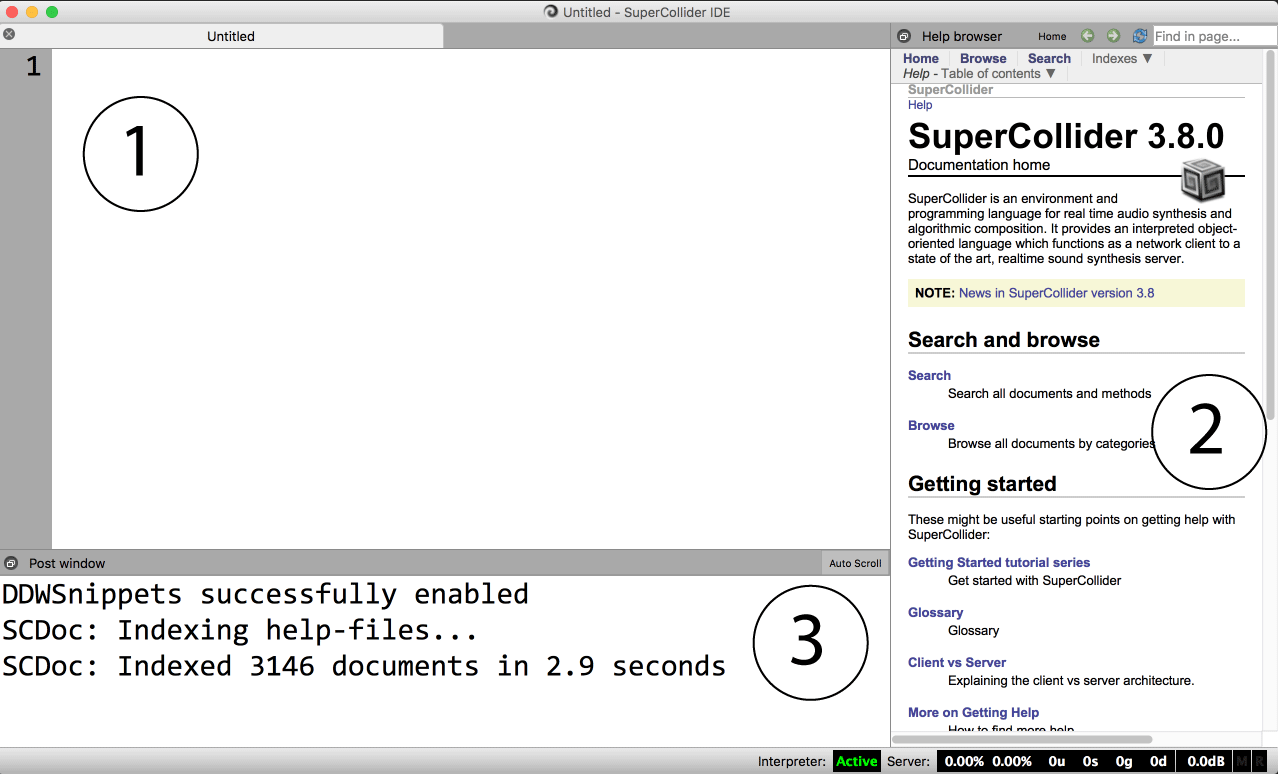
\includegraphics[scale=0.18]{interface1}
\centering
\caption{La interface}
\label{fig:áreas}
\end{figure}

Podemos configurar el modo en el que queremos ordenar esta interface haciendo click en el menú de cada ventana:

\begin{figure}[h]
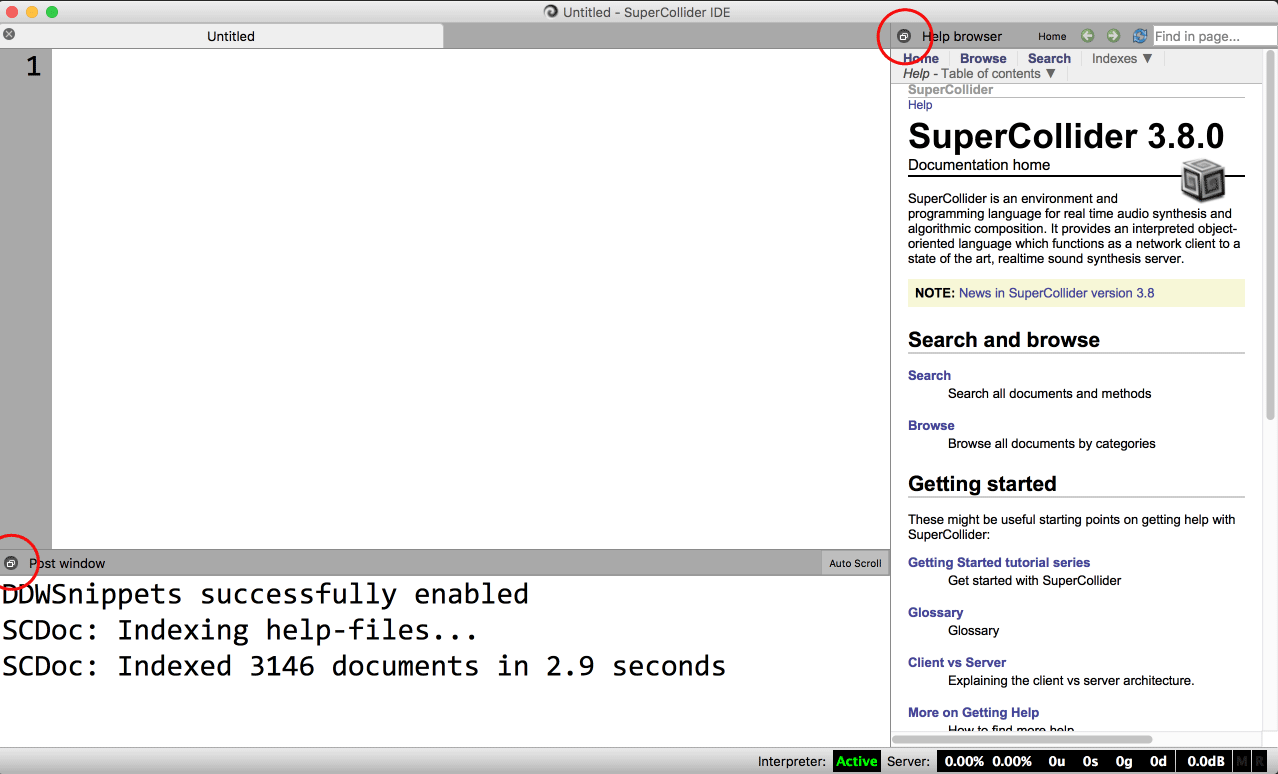
\includegraphics[scale=0.18]{interface2}
\centering
\caption{Orden de elementos}
\label{fig:orden}
\end{figure} 

\begin{itemize}
	\item Undock/Dock: monta y desmonta la ventana. Podemos arrastrarla y situarla en el sitio desado.
	\item Detach/Attach: crea una ventana flotante independiente.
	\item Close: cierra la ventana.
	\label{fig:docklets}
\end{itemize}

Si cerramos una de estas ventanas por accidente, podemos recuperarla yendo a la pestaña view/docklets:

\begin{figure}[h]
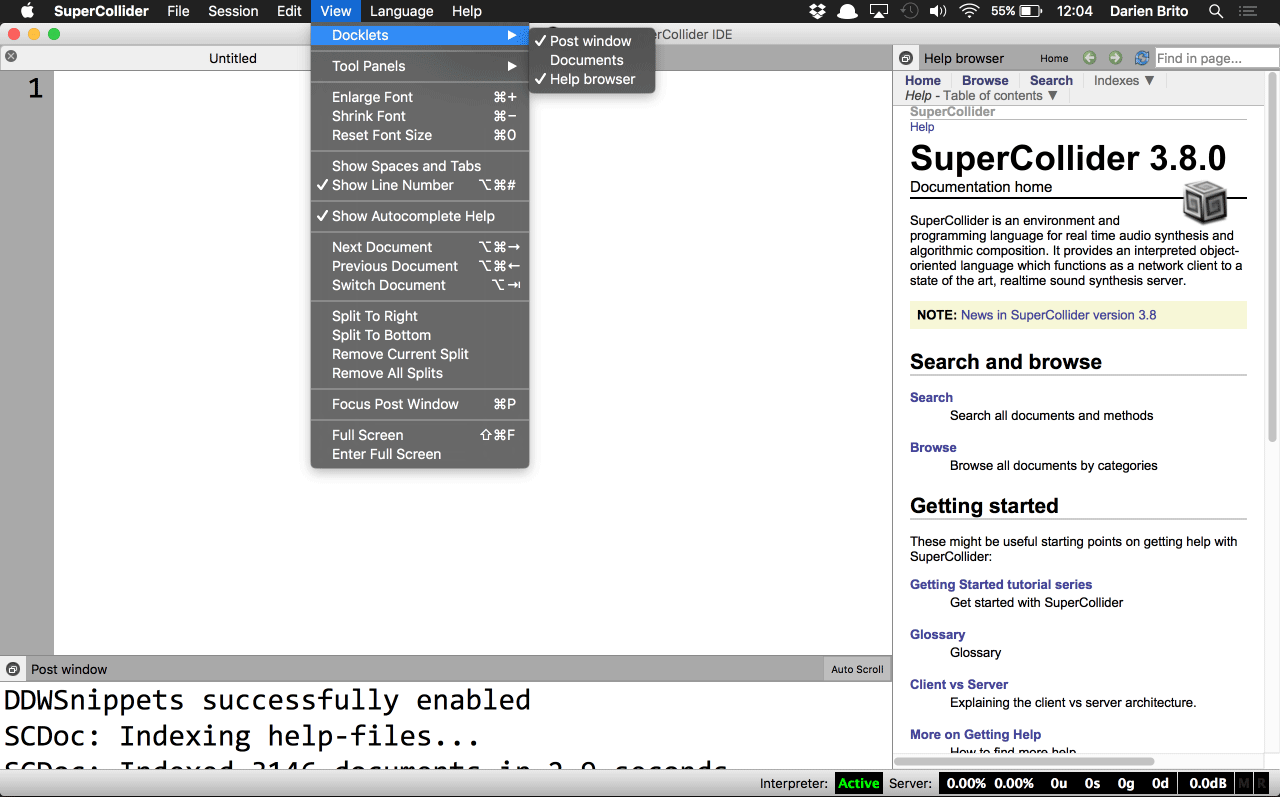
\includegraphics[scale=0.18]{interface3}
\centering
\caption{Activar docklets}
\label{fig:activar}
\end{figure} 

``Post window'' es nuestra consola y ``Help browser'' nuestra ventana de ayuda. ``Documents'' es un menú adicional que nos permite ver el directorio actual del documento en el que estamos trabajando.

Si queremos alterar los colores de la interface, podemos ir a: \\
SuperCollider/preferences/editor/Fonts\&Colors y escoger la configuración deseada. En el caso de este tutorial, yo he escogido el preset \textit{Black} y la fuente \textit{consolas}.

\section{Nociones preliminares}

Finalmente, aquí una guía con síntaxis y objetos que veremos en nuestro curso introductorio. Si la explicación en esta guía no tiene mucho sentido en este momento no hay problema. Esta aquí para prepararte y se complementa con las explicaciones del vídeo. 

\begin{itemize}

\item \textbf{Integer}: un número íntegro. ej: 1, 10, 100

\item \textbf{Float}: un número decimal. ej: 1.0, 10.0, 100.0

\item \textbf{String}: una cadena de caracteres, palabras, frase, oración o una secuencia ordenada de longitud arbitraria. Se crean con los símbolos para comillas `` ''. Por tanto, todo dentro de estos símbolos se convierte en una String, incluso números. ej: ``hola'', ``otra cosa'', ``123.1''.

\item \textbf{Comentarios}: texto que no es evaluado por el intéprete. Se usan para dejar notas o aclaraciones en un programa. Se crean con los símbolos: 
\begin{verbatim} 
// 
\end{verbatim}
Todo lo posterior a estos símbolos se convierte en un comentario a menos que creemos una nueva linea. A traves de nuestro tutorial, encontrarás varios comentarios que aclaran líneas de código. ej:

\begin{verbatim} 
SinOsc.ar() // este es un oscilador sinusoide
\end{verbatim}

Para comentarios multi-línea podemos usar los símbolos:

\begin{verbatim} 
/*   */ 
\end{verbatim}

Todo lo que va dentro de estos símbolos se convierte en un comentario. ej:

\begin{verbatim} 
/*
Todo esto es un comentario.

Puedo crear varias líneas.
*/
\end{verbatim}

\item \textbf{Array}: una colección de elementos. Un Array se crea con los símbolos: 
\begin{verbatim} 
[ ] 
\end{verbatim} 
Un array sirve para almacenar varios objetos en una sola caja, por así decirlo. Podemos acceder a los elementos de esta caja usando un número índice, que es la posición del objeto en el Array. ej: 
\begin{verbatim} 
[1, 10.0, ``hola''] 
\end{verbatim}

\item \textbf{Punto y coma (;)}: El punto y coma sirve para decirle al intérprete que una instrucción determinada a concluido. A través de los programas que escribamos verás como separar instrucciones usando este símbolo.

\item \textbf{var}: una variable. Se usa para referirnos a un objeto usando una palabra clave arbitraria. Esta palabra puede ser cualquier cosa siempre y cuando no inicie con mayúsculas o números y no tenga caracteres especiales como acentos. Para asignar un valor a una variable, usamos los signos de igual. ej: 

\begin{verbatim} 
var miVariable = 10;
\end{verbatim}

\item \textbf{postln}: un método. Métodos son funciones que los objetos entienden a fin de realizar una acción. El método postln se encarga de imprimir el objeto en la consola. Para usar un método, necesitamos usar antes un punto, a fin de que el intérprete sea capaz de entender en donde inicia el método. ej: 

\begin{verbatim} 
``¡Hola Mundo''.postln;
\end{verbatim}

\item \textbf{Funciones}: una función es una serie de instrucciones encapsuladas en un objeto. Se usan cuando queremos crear porciones de código re-utlizables. Se crean con los símbolos:

 \begin{verbatim} 
{ }
\end{verbatim}

Podemos asignar una función a una variable y reutilizarla a través de nuestro programa. ej:

\begin{verbatim} 
var f = { ``Hola mundo''.postln };
\end{verbatim}

Para evaluar una función usamos el método value. ej:

\begin{verbatim} 
f.value;
\end{verbatim}

\item \textbf{arg}: un argumento. Se usa para crear una compuerta a través de la cual pasar un objeto. Usamos argumentos cuando tenemos funciones que requieren valores flexibles para operar. ej: 

\begin{verbatim} 
var f = {arg i; i.postln }; // imprime el objeto en la consola
f.value(1); // imprime 1
f.value(10); // imprime 10
\end{verbatim}

\end{itemize}

\section{Usando los documentos de soporte}

Como ya hemos dicho, existen documentos de soporte en el \href{
https://github.com/DarienBrito/Quadro_SCIntro}{\textbf{repositorio}} de nuestro tutorial. La idea de estos documentos es que tengas a la mano todo lo que vamos viendo en cada vídeo. Te recomiendo realizar variaciones de cada ejercicio en los documentos por tu cuenta, a fin de entender los conceptos tal y como se van presentando. Para este propósito, he dejado un espacio entre líneas de código, de modo que te invite a experimentar un poco.

Te deseo buena suerte con este tutorial y espero que la información que encuentres te sea de ayuda. No dudes en escribir a la dirección dada en la plataforma con sugerencias o comentarios. ¡Feliz programación!



\end{document}

